\begin{center}
    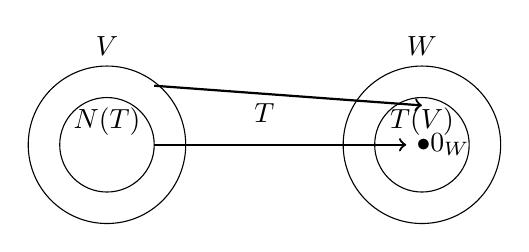
\begin{tikzpicture}
    \draw (1,0) ellipse (1cm and 1cm) node[above] {$\mathscr{N}(T)$};
    \draw (5,0) ellipse (1cm and 1cm);
    \draw (5,0) ellipse (0.6cm and 0.6cm) node[above] {$T(V)$};
    \draw (1,0) ellipse (0.6cm and 0.6cm);
    \draw (5,1.25) node {$W$};
    \draw (3,0.4) node {$T$};
    \draw (1,1.25) node {$V$};
    \draw[thick,->] (1.6,0) -- (4.8,0) node[right] {$\bullet\Vec{0}_W$};
    \draw[thick,->] (1.6,0.75)--(5.0,0.5);
    \end{tikzpicture}
\end{center}